% DAC 2027 research manuscript format, checked against the official CFP on
% 2026-10-29. This is an explicitly hypothetical-results design draft.
% No invented numbers in this file may be promoted to measured evidence.
\documentclass[conference,9pt,letterpaper]{IEEEtran}
\usepackage[T1]{fontenc}
\usepackage{newtxtext,newtxmath}
\usepackage{graphicx}
\usepackage{booktabs}
\usepackage{amsmath}
\usepackage{array}
\usepackage{xcolor}
\usepackage{cite}
\usepackage{url}
\usepackage[hidelinks]{hyperref}
\usepackage{eso-pic}
\usepackage{stfloats}
\usepackage{balance}
\usepackage{soul}
% Yellow: hypothetical/pending. Blue: AI disclosure. Keep semantic notices.
\definecolor{DraftYellow}{RGB}{255,242,153}
\definecolor{AIBlue}{RGB}{207,234,250}
\newcommand{\draftnote}[1]{{\sethlcolor{DraftYellow}\hl{#1}}}
\newcommand{\draftvalue}[1]{{\setlength{\fboxsep}{0.4pt}\colorbox{DraftYellow}{#1}}}
\newcommand{\ainote}[1]{{\sethlcolor{AIBlue}\hl{#1}}}
\hypersetup{pdftitle={MECC: Single-GPU MoE Inference with Compiler-Guided Three-Tier Expert Caching -- Hypothetical Design Draft},pdfauthor={},pdfsubject={All evaluation outcomes are hypothetical design targets, not measurements. Not for submission.},pdfkeywords={MoE, single GPU, three-tier cache, hypothetical results}}
\AddToShipoutPictureFG{\AtPageLowerLeft{\put(45,18){\makebox(520,12){\normalfont\fontsize{8}{9}\selectfont\color{brown}\draftnote{HYPOTHETICAL RESULTS DESIGN DRAFT --- NOT MEASURED --- NOT FOR SUBMISSION}}}}}
\newcommand{\mecc}{\textsc{MECC}}
\newcommand{\BH}{B_{\mathrm H}}
\newcommand{\BC}{B_{\mathrm C}}
\newcommand{\KH}{K_{\mathrm H}}
\newcommand{\KC}{K_{\mathrm C}}
\newcommand{\scenario}{\draftnote{Hypothetical evaluation.}}
\newtheorem{proposition}{Proposition}
\title{MECC: Single-GPU MoE Inference with\protect\\Compiler-Guided Three-Tier Expert Caching}
% Anonymous review copy: no author names or affiliation spacer rows.
\author{}
\begin{document}
\maketitle
\begin{abstract}
We study single-GPU mixture-of-experts inference under task memory caps that prevent full expert residency in HBM and host memory. SSD delivery then stalls computation. MECC combines profile-guided placement, cross-tier retention, and dependency-aware transfers. Its design preserves selected experts and FP16 weights. \draftnote{Illustrative targets specify} \draftvalue{$1.25$}--\draftvalue{$1.42\times$} speedup over a local SSD-native adapter, rather than a reproduction of a published system. A single-GPU target takes \draftnote{eight seconds per token}; a two-GPU resident target takes \draftvalue{2.8} seconds. The evaluation separates allocation feasibility from latency and nominal GPU-time. Measurements and matched external comparisons remain necessary to establish the design's benefit.
\end{abstract}
\begin{IEEEkeywords}
Mixture of experts, single-GPU inference, expert offloading, three-tier caching, hardware/software co-design.
\end{IEEEkeywords}

\section{Introduction}
Mixture-of-experts (MoE) models select a subset of experts for each token~\cite{shazeer,switch,gshard}. Mixtral and DeepSeekMoE instantiate sparse routing in language models~\cite{mixtral,deepseekmoe}. A single GPU can execute selected experts without full HBM residency, provided each weight is delivered before computation.

Shared servers assign each service a host-memory allowance. When combined HBM and host residency cannot hold the expert pool, requests reach SSD. FlexGen and DeepSpeed Inference already plan heterogeneous-memory execution~\cite{flexgen,dsinference}; flash-aware inference also addresses models exceeding DRAM~\cite{llmflash}. We study expert delivery under fixed task caps.

Prior work uses CPU/GPU orchestration~\cite{fiddler}, memory-constrained planning~\cite{lightning}, and SSD-native delivery~\cite{ssdllama}. MoE-Infinity traces activations for cache replacement and prefetch~\cite{moeinfinity}. ProMoE predicts future expert use~\cite{promoe}. Learned replacement~\cite{flashmoe} and domain-guided residency~\cite{core} further exploit routes. We compare placement, retention, and scheduling under common physical caps.

Three coupled decisions govern expert delivery. \textbf{First, capacity has to be distributed across layers.} Uniform slots can leave some layers repeatedly reading from SSD. \textbf{Second, HBM eviction has to preserve later reuse.} A fixed CPU pool may discard useful experts, while independent tier caches can retain duplicate copies. \textbf{Third, residency has to track request changes.} An initial profile covers startup demand; online observations update that placement as the working set changes.

Our design treats the route profile as an initial residency prior and actual requests as online corrections. \mecc{} assigns these roles across HBM, CPU pinned memory, and SSD. The compiler assigns expert rankings and layer capacities. The runtime promotes requested experts and demotes HBM victims into the host working set. Transfer overlap requires independent work and enforced readiness before computation. Section~\ref{sec:overview} presents the framework; Section~\ref{sec:implementation} separates its contract from the current prototype.

We ask whether a profile prior improves finite-horizon service beyond the same retention and delivery machinery. Component controls separate capacity allocation, initialization, and overlap. The resource comparison includes the smallest feasible resident allocation. \draftnote{All numerical outcomes below are authored scenarios.}

\section{Deployment Model and Challenges}
\label{sec:challenges}
\subsection{Single-GPU Execution with Bounded Host Memory}
Consider $L$ MoE layers. Layer $\ell$ contains $N_\ell$ experts and selects $k_\ell$ per token. Expert $e=(\ell,j)$ is an immutable weight object of size $s_e$. The GPU also stores dense weights, activations, the KV cache, and temporary buffers. The expert-residency allowance is $\BH$; the total task-level host allowance is $\BC$. Host mirrors and staging buffers count toward $\BC$.

Let $\bar B_{\mathrm H}$ and $\bar B_{\mathrm C}$ denote unique expert-residency capacities after charging other allocations. The target regime satisfies $\sum_e s_e>\bar B_{\mathrm H}+\bar B_{\mathrm C}$ and exceeds the task host allowance. Post-initialization SSD demand traffic measures its operational impact; startup reads alone do not establish this regime. Models that fit in host memory serve as two-tier controls. Models that fit in HBM need no expert offloading.

An HBM hit uses resident weights. A CPU hit requires host-to-device (H2D) transfer. An SSD miss adds an SSD-to-host read. We record the expert's tier when demand arrives, before servicing the request. Separate counters record physical SSD and transfer traffic, including prefetches.

\subsection{Challenge 1: Allocate Capacity across Layers}
The value of a cache slot depends on the layer's request distribution and miss cost. A small working set needs few slots. A broader working set can cause repeated cold reads under the same allocation. This difference motivates moving capacity between layers while holding total memory fixed.

Figure~\ref{fig:challenges}(a) illustrates four representative layers sharing 16 equal-size CPU slots. Uniform allocation assigns four slots per layer; profile-guided allocation assigns two, three, five, and six. HBM capacity and replacement are fixed. \draftnote{The hypothetical plan} moves slots toward layers with greater SSD demand. The first two layers lose coverage while the last two gain it. The measured counterpart must report request-weighted aggregate misses, rather than averaging percentages with different denominators.

\subsection{Challenge 2: Preserve Reuse after HBM Eviction}
An expert can be requested again soon after HBM eviction. A fixed CPU pool retains only its predefined members. Independent tier caches may instead retain copies of the same expert. These policies differ in both reuse coverage and physical duplication.

Figure~\ref{fig:challenges}(b) illustrates a fixed CPU pool, independent LRU, and MECC retention. These names identify retention rules, not distinct published implementations. The missing control is exclusive LRU with matching per-layer combined capacities and initial stacks, accompanied by duplicate-byte and migration measurements. Figure~\ref{fig:retention} illustrates the state changes.

\subsection{Challenge 3: Initialize Residency and Track Changes}
A profile supplies access information before the first request. Online history tracks changes after service begins. Fixed placement can become stale when the working set shifts. An online policy without a profile first has to discover that working set. Their combination targets startup misses and later adaptation.

The required experiment crosses profile/random initialization with static/adaptive residency. Figure~\ref{fig:challenges}(c) illustrates three of these four configurations across an authored shift. \draftnote{The fourth configuration, profile cost, no-shift control, uniform access, and mismatched profiles remain unmeasured.} These curves specify a hypothesis about startup and adaptation; they do not establish natural routing drift.

\begin{figure*}[tb]
\centering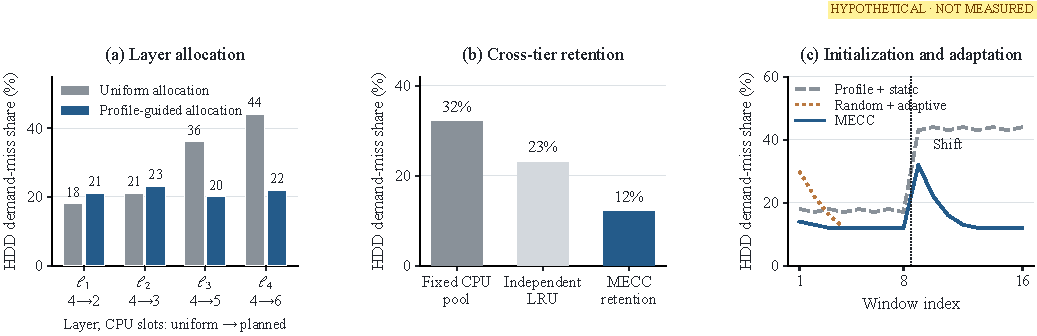
\includegraphics[width=\textwidth]{ideal_figures/fig02_challenges.pdf}
\caption{Deployment challenges. (a) Four representative layers share 16 equal-size CPU slots; tick labels show uniform $\rightarrow$ planned slots. (b) Fixed CPU pool, independent LRU, and MECC retention under the same profile. (c) Profile + static, random + adaptive, and profile + adaptive (MECC) across a shift. Random + static is not plotted. \textbf{\draftnote{All values and windows are hypothetical.}}}
\label{fig:challenges}
\end{figure*}

\section{Overview}
\label{sec:overview}
\begin{figure*}[!b]
\centering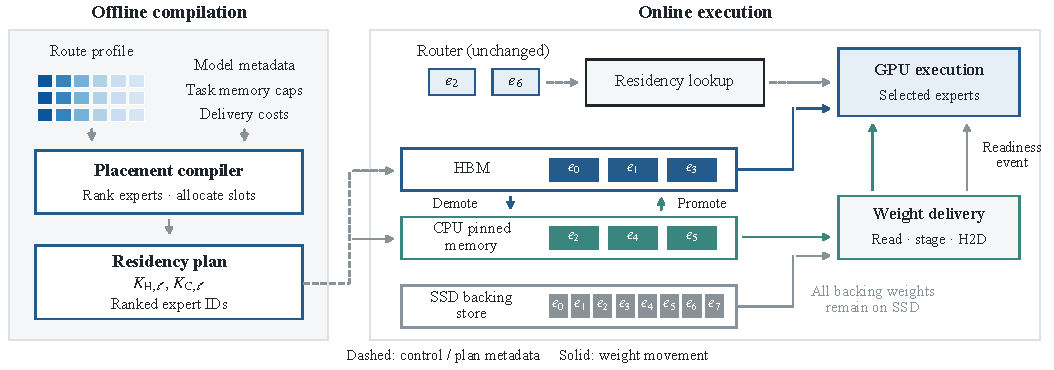
\includegraphics[width=\textwidth]{figures/fig01_overview.pdf}
\caption{\mecc{} framework. Offline compilation emits capacities $K_{\mathrm H,\ell}$ and $K_{\mathrm C,\ell}$ and ranked expert IDs. Online lookup resolves unchanged router selections against HBM, CPU pinned memory, and SSD. Weight delivery records a readiness event before GPU execution. Dashed arrows carry control/plan metadata; solid arrows move weights. Expert IDs and occupancy are schematic.}
\label{fig:overview}
\end{figure*}

Figure~\ref{fig:overview} separates offline compilation from online execution. An independent route profile, model metadata, task memory caps, and delivery costs define the compilation inputs. The output specifies layer capacities and initial expert IDs. Mirrors and staging are charged outside unique primary residency; SSD retains all backing weights.

The unchanged router supplies demand IDs. Residency lookup selects a source tier; the runtime promotes requested experts and demotes HBM victims. The delivery path enforces weight readiness before execution. Layer capacities stay fixed during a run, while expert identities and recency change. Planner controls therefore fix online rules; replacement controls fix quotas and initialization (Section~\ref{sec:mechanisms}).

\section{Method}
\label{sec:method}
\subsection{Compiler: Profile-Guided Placement}
The compiler takes model metadata, memory budgets, delivery costs, and an independent route profile. The profile supplies request probability $p_e$ for each expert. For equal-size experts within a layer, a discrete Zipf model summarizes the ranked probabilities:
\begin{equation}
 q_{\ell,r}=\frac{r^{-\alpha_\ell}}{H_{N_\ell}(\alpha_\ell)},\qquad
 H_n(\alpha)=\sum_{r=1}^{n}r^{-\alpha}.
\end{equation}
Here $q_{\ell,r}$ is conditional on an expert selection in layer $\ell$. Let $w_\ell$ be that layer's fraction of all selections. The global probability is $p_e=w_\ell q_{\ell,r}$, with $\sum_\ell w_\ell=1$. For fixed top-$k$ routing, $w_\ell=k_\ell/\sum_j k_j$. Each rank retains its profiled expert ID. Empirical probabilities can replace the fitted Zipf distribution. Neither representation encodes request order.

Let $x_{e,t}\in\{0,1\}$ indicate the primary tier of expert $e$. The tiers are HBM, CPU, and SSD, denoted by $\mathrm H$, $\mathrm C$, and $\mathrm S$. Residency budgets $\bar B_t$ must exclude buffers and mirrors. The following static objective is a reference model, not a claim that the current planner solves the full problem:
\begin{align}
 \min_x\quad &\sum_e p_e\sum_t x_{e,t}T_t(s_e),\label{eq:placement}\\
 \text{s.t.}\quad&\sum_t x_{e,t}=1,\quad
 \sum_e s_e x_{e,t}\le \bar B_t\quad(t\in\{\mathrm H,\mathrm C\}).\nonumber
\end{align}
The affine model $T_t(s)=a_t+s/b_t$ represents fixed overhead and effective bandwidth. Calibration uses the target machine. Equation~\ref{eq:placement} estimates static delivery cost under the profile. Runtime locality, migration, and overlap are evaluated separately.

\begin{proposition}
Assume equal-size objects, fixed request probabilities, independent tier capacities, and $T_{\mathrm H}\le T_{\mathrm C}\le T_{\mathrm S}$. An optimal static placement fills HBM with the most probable objects, CPU with the next most probable objects, and SSD with the remainder.
\end{proposition}
\noindent\emph{Proof sketch.} Suppose $p_i>p_j$ and object $i$ occupies the slower tier. Exchanging the two objects changes expected cost by $(p_i-p_j)(T_{\mathrm{fast}}-T_{\mathrm{slow}})\le0$. Repeated exchanges produce ranked placement. Filling an empty faster-tier slot also cannot increase cost. The result applies to the stated static model.

The multilayer implementation allocates slots by marginal coverage. Under the Zipf model, a slot covering rank $r$ adds
\begin{equation}
 \Delta_{\ell}(r)=w_\ell q_{\ell,r}.
\end{equation}
This is a coverage score, not the exact latency marginal of Equation~\ref{eq:placement}. Tier-boundary movements can affect both HBM and CPU assignments. The intended heuristic allocates HBM slots first, then CPU slots from the remaining ranks. At each step it selects the largest next-rank score; ties use layer ID. Expert-ranking ties use expert ID. It stops at the tier's slot cap or exhaustion of experts. Per-layer minima, if enabled, are assigned first and an infeasible minimum allocation must be rejected. A direct scan costs $O(L(S_{\mathrm H}+S_{\mathrm C}))$ after ranking, where $S_t$ is a total slot cap. These validation rules describe the required planner contract; the prototype does not yet enforce all of them. Batched prefill additionally requires distinguishing token selections from distinct expert fetches. The sequential heuristic does not solve the general static objective.

The plan records per-layer capacities, ranked expert IDs, initial tiers, and modeled hit fractions. Input model/profile hashes, object sizes, and the ranking mode identify its provenance. A missing profile requires an explicitly labeled natural-order fallback. It cannot silently stand in for profile-guided placement. Initialization traffic and planning time are charged before comparing finite service horizons.

\subsection{Runtime: Cross-Tier Retention}
Each layer has ordered HBM and CPU residency maps. An HBM hit updates recency. A CPU hit removes the expert from CPU residency and promotes it to HBM as most recently used. An SSD miss reads the weights into staging before H2D transfer. When HBM is full, its least-recently used expert is demoted to CPU. CPU pressure evicts the least-recently used host resident. The SSD backing weights remain available.

Figure~\ref{fig:retention} starts with HBM $[e_0,e_1]$ and CPU $[e_2,e_3,e_4]$. Requesting $e_2$ promotes it and demotes $e_0$. The next request for $e_0$ hits CPU. This example uses exclusive logical residency. An implementation can keep a CPU mirror to avoid device-to-host (D2H) transfer on eviction. The mirror consumes host memory and is charged separately.

\begin{figure}[t]
\centering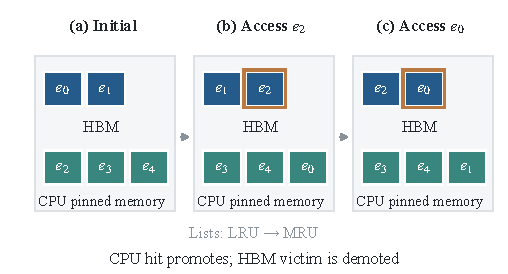
\includegraphics[width=\columnwidth]{figures/fig03_retention.pdf}
\caption{Cross-tier retention with two HBM slots and three CPU slots. Lists run from LRU to MRU. A CPU hit promotes the requested expert and makes room for the HBM victim. Mirrors and staging consume additional physical space. Schematic.}
\label{fig:retention}
\end{figure}

For a serial demand stream within one layer, concatenate the HBM MRU-to-LRU stack with the CPU MRU-to-LRU stack. Exclusive promotion and victim demotion preserve the corresponding LRU stack of capacity $\KH+\KC$. This reference requires matching initialization, no prefetch or alternative admission, and completed transitions before the next request. It does not imply equivalence to a cache that reallocates capacity across layers, or dominance over static placement.

\subsection{Delivery: Dependency-Aware Overlap}
A correct asynchronous implementation requires a readiness event after each pinned-host copy. The computation stream must wait before consuming the weight. The source buffer must remain live until copy completion, and the resident weight until its last consumer finishes. These are required lifetime rules, including across separate loading and dispatch iterators; the prototype's current asynchronous path is not yet validated against them.

At batch one, routing reveals the selected IDs only after the current layer's gate. Copying one selected expert may overlap computation of another already-ready expert if kernel and aggregation order permit. This provides no knowledge of a later layer's route. In-flight weights must be protected from eviction. Replacement comparisons must disable predictive prefetch; the overlap control must hold admission, residency, and requests fixed. The available overlap and its exposed critical path remain measurements, rather than an assumed gain from a copy stream.

Figure~\ref{fig:delivery} pairs one HBM-resident expert with one SSD-backed expert from the same gate. SSD read precedes H2D and readiness. Copy completion releases the pinned source; final-consumer completion permits GPU eviction. Useful independent computation determines the available overlap.

\begin{figure}[t]
\centering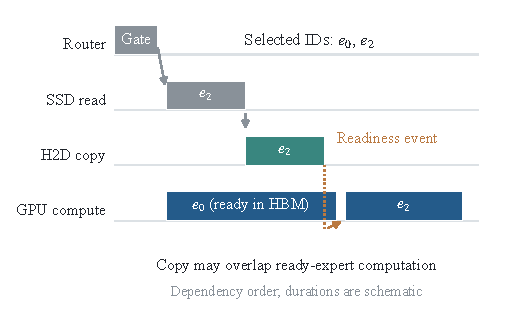
\includegraphics[width=\columnwidth]{figures/fig08_delivery.pdf}
\caption{Delivery dependencies after a gate selects $e_0$ and $e_2$. The resident $e_0$ can execute while $e_2$ is read and copied. The readiness event protects consumption of $e_2$. Kernel order is unchanged. Durations are schematic; the figure asserts no measured overlap.}
\label{fig:delivery}
\end{figure}

The design requires unchanged weights, selected experts, kernels, and aggregation order. Under these conditions, changing residency preserves the forward computation. The implementation also needs correct synchronization. The validation protocol compares synchronous and asynchronous paths on identical inputs using weight hashes, route selections, logits, tokens, and perplexity; \draftnote{these tests remain to be executed.}

\section{Implementation}
\label{sec:implementation}
Model adapters map layer/expert IDs to weight objects, and policies share an end-to-end loader. \draftnote{Implementation validation remains pending.} The current harness requires reconciliation of synthetic layer exponents, optional co-occurrence ranking, CPU mirrors, readiness events, and phase-mixed counters with Section~\ref{sec:method}. No GPU validation is reported as completed.

Physical accounting deduplicates storage identities, not expert IDs: distinct live copies still consume bytes. Let $R_t$ be resident expert bytes, $D_{\mathrm H}$ distinct host mirrors, $S_t$ staging, and $O_t$ other charged allocations. The required constraints are
\begin{align}
 R_{\mathrm C}+D_{\mathrm H}+S_{\mathrm C}+O_{\mathrm C}&\le B_{\mathrm C},\\
 R_{\mathrm H}+W_{\mathrm{dense}}+W_{\mathrm{KV/act}}+S_{\mathrm H}+O_{\mathrm H}&\le B_{\mathrm{GPU}}.
\end{align}
Full mirroring requires $D_{\mathrm H}\ge R_{\mathrm H}$. \draftnote{The archived 42 GB HBM-expert / 6 GB mirror example is withdrawn as infeasible under full mirroring and a 40 GB host cap.} Residency must be reduced or a mirror-free path validated. Peak measurements must include initialization and transient copies, not only steady residency.

Counters must separate initialization, warmup, prefill, decode, and quality evaluation. TPOT divides decode time by measured intervals; TTFT includes prefill and the first output. Demand-miss share is the fraction of selected-expert arrivals without ready HBM/CPU weights. In-flight prefetch is logged separately. Physical SSD/H2D/D2H bytes use the same phase boundaries. \draftnote{The current phase-mixed counters require replacement.}

\begin{figure*}[tb]
\centering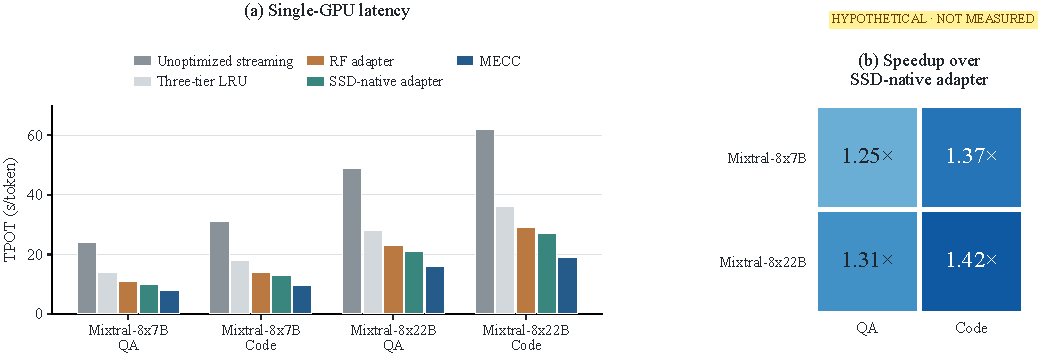
\includegraphics[width=\textwidth]{ideal_figures/fig04_performance.pdf}
\caption{\textbf{\draftnote{Hypothetical performance.}} (a) TPOT for single-A100 policies. RF adapter and SSD-native adapter are local mechanisms, not published-system measurements. Nominal allowances are 50~GB for experts and 40~GB for host memory; physical feasibility remains unverified. (b) Speedup over SSD-native adapter, calculated from the same TPOT targets. Targets have no error bars.}
\label{fig:performance}
\end{figure*}

\section{Evaluation}
\label{sec:evaluation}
\scenario{} \draftnote{All results and quality checks below are authored targets. They are not measurements.} Budget feasibility and implementation correctness are prerequisites, not established outcomes.

\subsection{Experimental Methodology}
\textbf{Models and workloads.} The scenario uses Mixtral-8x7B and Mixtral-8x22B~\cite{mixtral,mixtral22} with question-answering and code prompts. One A100 provides 80~GB of physical HBM. The nominal expert allowance is 50~GB, subject to total-peak checks. The task host cap is 40~GB. Profile and evaluation splits are independent. Main comparisons use batch one, 128 input tokens, 128 output tokens, and deterministic decoding. \draftnote{Dataset, model, and input revisions remain to be frozen for execution.}

\textbf{Unoptimized streaming.} This baseline executes the same selected FP16 experts on one GPU, sharing the model, tokenizer, kernels, SSD-read semantics, and task caps with \mecc{}. Demand staging disables profile placement, dynamic CPU retention, and overlap. Report its default residency and achieved occupancy; equal caps alone do not establish an equally provisioned comparison.

\textbf{Cache baselines.} Three-tier LRU controls for basic caching. \draftnote{RF and SSD-native are hypothetical local mechanism adapters.} The recency/frequency (RF) adapter uses a heuristic whose precise rule remains to be frozen; FlashMoE~\cite{flashmoe} learns a predictor from these signals. SSD-native represents three-tier residency motivated by SSD-LLaMA~\cite{ssdllama}. Neither establishes a reproduction of the cited system. Versioned external runs, including MoE-CORE~\cite{core}, remain separate experiments.

\textbf{Multi-GPU reference.} The resident reference partitions the full FP16 model across two, four, or eight A100s where capacity permits. It uses matched inputs and decoding without SSD delivery. Its resource record includes GPU count, parallelism, interconnect, software revision, and memory peak. \draftnote{The eight-GPU point is an authored scenario reference, independent of the cited systems.}

\textbf{Metrics.} We report TPOT, TTFT, throughput, demand-miss share, SSD/H2D/D2H bytes, and physical memory peaks. GPU-time comparisons use the same workload. \draftnote{We omit authored repeat variation from the plots.} Execution must report independent repeats, request-level distributions, and the statistic used for uncertainty. \draftnote{No uncertainty estimate is available in this draft.}

\subsection{Latency under Matched Single-GPU Budgets}
Figure~\ref{fig:performance}(a) fixes one A100 and the task host cap across four model/workload combinations. Scenario TPOT is \draftvalue{8.0}, \draftvalue{9.5}, \draftvalue{16.0}, and \draftvalue{19.0}~s for \mecc{}, versus \draftvalue{24}, \draftvalue{31}, \draftvalue{49}, and \draftvalue{62}~s for unoptimized streaming. These values correspond to \draftvalue{$3.00\times$}, \draftvalue{$3.26\times$}, \draftvalue{$3.06\times$}, and \draftvalue{$3.26\times$} speedup. This comparison targets the complete stack. Section~\ref{sec:mechanisms} shows cumulative additions; independent attribution remains untested.

SSD-native adapter takes \draftvalue{10}, \draftvalue{13}, \draftvalue{21}, and \draftvalue{27}~s per token. Figure~\ref{fig:performance}(b) gives the corresponding \draftvalue{$1.25$}--\draftvalue{$1.42\times$} gains. This is the closer local cache comparison; the larger streaming gain does not establish an advantage over other cache systems.

Scenario TTFT is \draftvalue{60/68/96/112}~s for \mecc{} and \draftvalue{130/155/230/280}~s for streaming. These values describe first response. TPOT describes later token intervals. Initialization is charged separately in the cost analysis below.

\subsection{Latency versus GPU Allocation}
The resident reference has eight-GPU TPOT targets of \draftvalue{1.0/1.2/1.8/2.1}~s in the same workload order. Figure~\ref{fig:budget}(b) and Table~\ref{tab:gpu} include the smaller resident allocations. The single-GPU configuration targets offline service whose latency allowance permits the resulting delay.

Table~\ref{tab:gpu} includes every specified resident allocation. The two-GPU resident target is faster and uses fewer nominal GPU-seconds than single-GPU \mecc{}. The one-GPU configuration instead tests feasibility when only one GPU can be allocated. A suitable use case is offline generation with a declared latency allowance; \draftvalue{127} decode intervals at \draftvalue{8}~s take about \draftvalue{17} minutes. This does not establish GPU-time, energy, or monetary savings.

\begin{table}[t]
\caption{\draftnote{Hypothetical 8x7B deployment point; not measured.}}
\label{tab:gpu}\centering
\begin{tabular}{lrr}\toprule
Configuration & TPOT (s) & GPU-s/token\\\midrule
\mecc{}, \draftvalue{1} GPU & \draftvalue{8.0} & \draftvalue{8.0}\\
Resident, \draftvalue{2} GPUs & \draftvalue{2.8} & \draftvalue{5.6}\\
Resident, \draftvalue{4} GPUs & \draftvalue{1.65} & \draftvalue{6.6}\\
Resident, \draftvalue{8} GPUs & \draftvalue{1.0} & \draftvalue{8.0}\\\bottomrule
\end{tabular}
\end{table}

\subsection{Component and Mechanism Analysis}
\label{sec:mechanisms}
Figure~\ref{fig:ablation} adds components to streaming on the first workload. Profile placement reduces scenario TPOT from \draftvalue{24} to \draftvalue{18}~s. Retention reduces it to \draftvalue{11}~s. Overlap reduces it to \draftvalue{8}~s. Each change measures a component within that stack. Component interactions require additional leave-one-out and factorial comparisons.

SSD demand-miss shares are \draftvalue{46}\%, \draftvalue{33}\%, \draftvalue{20}\%, and \draftvalue{20}\%. Placement and retention reduce the illustrated SSD demand share. Overlap keeps the same miss share and reduces exposed waiting. The \draftvalue{12}\% target in Figure~\ref{fig:challenges}(b) belongs to a separate controlled trace.

Mechanism controls hold requests fixed. Separate controls must vary layer allocation and initial expert identities while holding the other fixed, and charge initial transfers. The retention comparison must record duplicate bytes under each policy. Within-phase shuffling preserves expert histograms and tests sensitivity to order. The shift scenario characterizes an authored workload; it provides no measured evidence of natural MoE drift.

Table~\ref{tab:controls} defines the comparisons needed for attribution. An allocation experiment redistributes quotas but retains the same ranking rule. An initialization experiment changes expert IDs within fixed quotas. The retention control uses identical primary capacities and initial stacks. The overlap control must preserve physical transfers as well as demand misses; equal miss percentages alone do not rule out extra I/O. \draftnote{These controls are specified, not completed results.}

\begin{table}[t]
\caption{Component controls. \draftnote{Execution remains pending.}}
\label{tab:controls}\centering
\begin{tabular}{@{}p{.19\columnwidth}p{.28\columnwidth}p{.43\columnwidth}@{}}\toprule
Component & Vary & Hold fixed\\\midrule
Allocation & Layer quotas & Ranking, online policy, bytes\\
Initialization & Initial expert IDs & Quotas, requests, online policy\\
Retention & Replacement rule & Quotas, initial stack, admission\\
Overlap & Schedule & Requests, transfers, kernel order\\\bottomrule
\end{tabular}
\end{table}

\begin{figure*}[tb]
\centering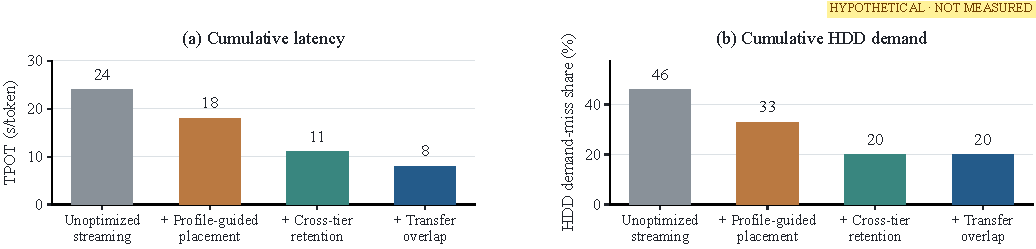
\includegraphics[width=\textwidth]{ideal_figures/fig05_ablation.pdf}
\caption{\textbf{\draftnote{Hypothetical ablation.}} (a) TPOT after adding each component. (b) SSD demand-miss share. The overlap-only step fixes admission, residency, and requests. Its miss share stays at \draftvalue{20\%}; exposed transfer time decreases.}
\label{fig:ablation}
\end{figure*}

\begin{figure*}[tb]
\centering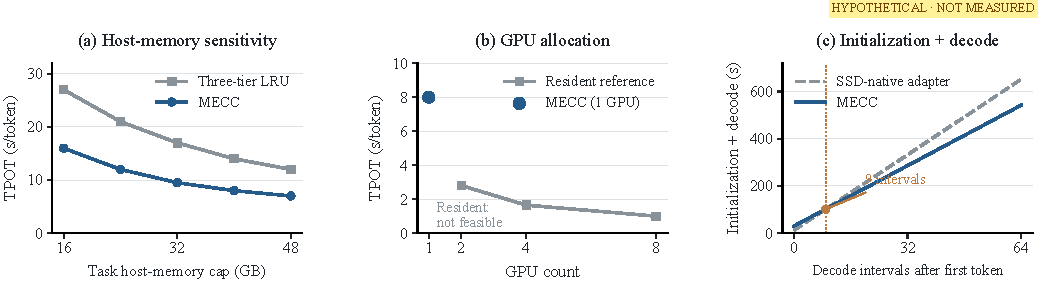
\includegraphics[width=\textwidth]{ideal_figures/fig06_budget_cost.pdf}
\caption{\textbf{\draftnote{Hypothetical sensitivity.}} (a) TPOT versus total task host cap. (b) Allocation comparison on 8x7B question answering; the full-model-resident reference exceeds one GPU. Only the single-GPU MECC design is specified. (c) Initialization plus decode intervals. \draftnote{An 18~s initial overhead and a 2~s/interval saving yield equality at nine intervals.} Additional loading, profiling, and prefill costs are outside this illustration.}
\label{fig:budget}
\end{figure*}

\subsection{Resource Sensitivity, Cost, and Quality}
\label{sec:resources}
Figure~\ref{fig:budget}(a) increases the host cap from \draftvalue{16} to \draftvalue{48}~GB on a fixed GPU. Scenario TPOT falls from \draftvalue{16} to \draftvalue{7}~s for \mecc{} and from \draftvalue{27} to \draftvalue{12}~s for conventional LRU. The paired curves compare residency at each task allowance. Each point requires independent physical accounting, including mirrors and buffers. These target curves do not establish feasibility under the stated cap.

Figure~\ref{fig:budget}(b) varies GPU count for 8x7B question answering. The resident configuration does not fit on one GPU. Its two-, four-, and eight-GPU targets are \draftvalue{2.8}, \draftvalue{1.65}, and \draftvalue{1.0}~s/token. Only the single-GPU \mecc{} target is shown. Earlier multi-GPU \mecc{} targets are withdrawn from the figure because this draft does not specify that extension. The smallest feasible resident reference must remain in the comparison.

Figure~\ref{fig:budget}(c) adds initialization to decode time. Initialization costs \draftvalue{30}~s for \mecc{} and \draftvalue{12}~s for the SSD-native adapter. Decode costs \draftvalue{8} and \draftvalue{10}~s/token, respectively. The plotted terms are equal at nine decode intervals after the first token. This is not a full-request crossover. For $n$ output tokens, full cost is $J(n)=I+\mathrm{TTFT}+(n-1)\mathrm{TPOT}$, with amortized profiling/loading included in $I$ and no double counting. The adapter TTFT and profile costs are unspecified, so no numerical full-request break-even follows.

The complete sensitivity matrix also varies HBM capacity, input/output lengths, batch size, and profile coverage or mismatch. Leave-one-out controls separate zero-copy eviction, pinning, batch H2D, and prefetching. A reverse resource comparison fixes a TPOT limit and finds each policy's minimum feasible host cap. \draftnote{These cases remain planned; the current curves cover only the displayed scenario points.}

The profile's service horizon matters. Its collection cost is charged once per frozen model/workload profile, then amortized over the requests that actually reuse it. A shorter horizon can favor the same runtime without profile initialization. Report planning time, initial SSD/H2D bytes, and request count before interpreting a steady-state TPOT gain. Cold-start and warm-service measurements answer different deployment questions.

\draftnote{The quality targets are identical weight hashes and expert selections, zero logit difference from deterministic synchronous execution, and zero perplexity difference on a fixed corpus.} \draftnote{These checks remain hypothetical.} Nondeterministic kernels require prespecified error tolerances and token comparisons. Weight checks and execution checks test separate properties.

\section{Related Work}
\label{sec:related}
\textbf{Sparse execution and serving.} Switch and GShard decouple active computation from total parameters~\cite{switch,gshard}; DeepSeekMoE uses fine-grained and shared experts~\cite{deepseekmoe}. DeepSpeed-MoE optimizes distributed inference~\cite{deepspeedmoe}; Tutel adapts parallelism/pipelining~\cite{tutel}; MegaBlocks targets sparse training kernels~\cite{megablocks}. PagedAttention and SGLang optimize KV allocation and prefix reuse~\cite{pagedattention,sglang}, distinct from expert residency.

\textbf{Heterogeneous memory.} ZeRO-Infinity uses GPU/CPU/NVMe for training~\cite{zeroinfinity}; DeepSpeed Inference supports heterogeneous serving~\cite{dsinference}. FlexGen plans tensor placement and throughput-oriented schedules~\cite{flexgen}. LLM in a flash combines reuse windows with flash-friendly layouts~\cite{llmflash}. PowerInfer splits hot/cold neuron computation across GPU/CPU~\cite{powerinfer}.

\textbf{Offloading.} Fast MoE offloading and SwapMoE target memory-constrained serving~\cite{offloading,swapmoe}. Fiddler uses popularity-based GPU placement and CPU expert computation~\cite{fiddler}. MoE-Lightning searches batching, execution, and weight/KV placement under CPU/GPU constraints, excluding disk variables~\cite{lightning}. Klotski combines expert-aware multi-batch execution with constraint-sensitive planning and correlation-aware prefetching~\cite{klotski}.

\textbf{Expert prediction.} Pre-gated MoE changes the gating design~\cite{pregated}; ProMoE predicts expert use from intermediate results~\cite{promoe}; MoE-Infinity uses activation traces for replacement/prefetch~\cite{moeinfinity}. MECC's demand-only control excludes prediction; its overlap control uses IDs available from the unchanged router.

\textbf{SSD-based serving.} SSD-LLaMA combines expert-pack I/O, lossless transport, frequency/recency-based VRAM admission, and RAM LRU~\cite{ssdllama}. Transient experts may bypass retention. FlashMoE learns a replacement predictor from recency/frequency signals and Belady-derived labels~\cite{flashmoe}. Plain RF/LRU omits these mechanisms.

\textbf{Coordinated residency.} MoE-CORE combines layer hit-rate curves, domain initialization, and routing history/scores~\cite{core}; optional substitution is separate from exact execution. ZipMoE combines lossless compression, compression-aware caching, and cache-affinity scheduling~\cite{zipmoe}. These overlaps require matched controls, not novelty claims based on module names.

The scope is SSD-active single-GPU serving. Local adapters do not establish superiority over these systems. \draftnote{Scenario outcomes require replacement measurements.}

\section{Conclusion}
\mecc{} combines profile-guided placement, cross-tier retention, and readiness-checked FP16 delivery for SSD-active single-GPU inference. \draftnote{The hypothetical evaluation} distinguishes fixed-budget latency from the GPU-allocation tradeoff. Matched competitors, component controls, physical peaks, and quality checks remain the required evidence.

\section*{\ainote{Content Generated by AI}}
\ainote{OpenAI Codex (GPT-6) assisted with text throughout, figure-generation code, and hypothetical outcomes. Human authors must verify the implementation, references, and replacement measurements before submission.}

% DAC 2027: at most six BODY pages, plus one REFERENCES-ONLY page.
% Build check verifies the actual boundary; do not shrink the IEEE margins.
\clearpage
\nobalance
\IEEEtriggeratref{15}
\bibliographystyle{IEEEtran}
\bibliography{references}
\end{document}
